\documentclass{beamer}\usepackage[]{graphicx}\usepackage[]{color}
% maxwidth is the original width if it is less than linewidth
% otherwise use linewidth (to make sure the graphics do not exceed the margin)
\makeatletter
\def\maxwidth{ %
  \ifdim\Gin@nat@width>\linewidth
    \linewidth
  \else
    \Gin@nat@width
  \fi
}
\makeatother

\definecolor{fgcolor}{rgb}{1, 0.894, 0.769}
\newcommand{\hlnum}[1]{\textcolor[rgb]{0.824,0.412,0.118}{#1}}%
\newcommand{\hlstr}[1]{\textcolor[rgb]{1,0.894,0.71}{#1}}%
\newcommand{\hlcom}[1]{\textcolor[rgb]{0.824,0.706,0.549}{#1}}%
\newcommand{\hlopt}[1]{\textcolor[rgb]{1,0.894,0.769}{#1}}%
\newcommand{\hlstd}[1]{\textcolor[rgb]{1,0.894,0.769}{#1}}%
\newcommand{\hlkwa}[1]{\textcolor[rgb]{0.941,0.902,0.549}{#1}}%
\newcommand{\hlkwb}[1]{\textcolor[rgb]{0.804,0.776,0.451}{#1}}%
\newcommand{\hlkwc}[1]{\textcolor[rgb]{0.78,0.941,0.545}{#1}}%
\newcommand{\hlkwd}[1]{\textcolor[rgb]{1,0.78,0.769}{#1}}%
\let\hlipl\hlkwb

\usepackage{framed}
\makeatletter
\newenvironment{kframe}{%
 \def\at@end@of@kframe{}%
 \ifinner\ifhmode%
  \def\at@end@of@kframe{\end{minipage}}%
  \begin{minipage}{\columnwidth}%
 \fi\fi%
 \def\FrameCommand##1{\hskip\@totalleftmargin \hskip-\fboxsep
 \colorbox{shadecolor}{##1}\hskip-\fboxsep
     % There is no \\@totalrightmargin, so:
     \hskip-\linewidth \hskip-\@totalleftmargin \hskip\columnwidth}%
 \MakeFramed {\advance\hsize-\width
   \@totalleftmargin\z@ \linewidth\hsize
   \@setminipage}}%
 {\par\unskip\endMakeFramed%
 \at@end@of@kframe}
\makeatother

\definecolor{shadecolor}{rgb}{.97, .97, .97}
\definecolor{messagecolor}{rgb}{0, 0, 0}
\definecolor{warningcolor}{rgb}{1, 0, 1}
\definecolor{errorcolor}{rgb}{1, 0, 0}
\newenvironment{knitrout}{}{} % an empty environment to be redefined in TeX

\usepackage{alltt}
\usepackage{../371g-slides}
\title{Correlation \& Simple Regression 2}
\subtitle{Lecture 10}
\author{STA 371G}
\IfFileExists{upquote.sty}{\usepackage{upquote}}{}
\begin{document}
  
  
  

  \frame{\maketitle}

  % Show outline at beginning of each section
  \AtBeginSection[]{
    \begin{frame}<beamer>
      \tableofcontents[currentsection]
    \end{frame}
  }

  %%%%%%% Slides start here %%%%%%%

  \begin{darkframes}
    \section{Regression basics}

    \begin{frame}
      \begin{center}
        
\includegraphics[width=3in]{add-health}

        \bigskip
        National Longitudinal Study of Adolescent to Adult Health

        \bigskip
        Nationally representative sample of US students in grades 7-12 were surveyed in the 1994-95 school year (\url{http://www.cpc.unc.edu/projects/addhealth})

        \bigskip
        Students were followed up on with subsequent in-home interviews four times (most recently 2008)
      \end{center}
    \end{frame}

    \begin{frame}
      This is an \textbf{awesome} data set, with data on:
      \begin{columns}[onlytextwidth]
        \column{.5\textwidth}
          \begin{itemize}
            \item family
            \item relationships
            \item health
            \item military service
            \item religion
            \item sex and STDs
            \item economics
            \item education
          \end{itemize}
        \column{.5\textwidth}
          \begin{itemize}
            \item personality
            \item criminality
            \item tobacco
            \item drugs
            \item alcohol
            \item pregnancy
            \item sleep
            \item daily activities
          \end{itemize}
      \end{columns}
    \end{frame}

    \begin{frame}
      \begin{center}
        Do people that start drinking younger tend to drink more (or less) when they become adults?
      \end{center}
      \bigskip\pause
      We want to know:
      \begin{itemize}[<+->]
        \item What is our best \textbf{prediction} of alcohol consumption if we know at what age they had their first drink?
        \item How good is that prediction?
        \item What is the \textbf{relationship} between alcohol consumption and age of first drink?
      \end{itemize}
    \end{frame}

    \begin{frame}
      \begin{tabular}{ll}
        Age of first drink & \textbf{Explanatory variable} ($X$) \\
        Number of drinks consumed as adult & \textbf{Response variable} ($Y$) \\
      \end{tabular}
    \end{frame}

    \begin{frame}[fragile]{Working with a large data set}
      Put the variables you will work with into a new data set in R; it's easier to work with and clean up that way.
\begin{knitrout}
\definecolor{shadecolor}{rgb}{0.137, 0.137, 0.137}\color{fgcolor}\begin{kframe}
\begin{alltt}
\hlstd{drinking} \hlkwb{<-} \hlkwd{data.frame}\hlstd{(}\hlkwc{age}\hlstd{=addhealth}\hlopt{$}\hlstd{h4to34,}
                       \hlkwc{num.drinks}\hlstd{=addhealth}\hlopt{$}\hlstd{h4to36)}
\end{alltt}
\end{kframe}
\end{knitrout}
    \end{frame}
    
    \begin{frame}[fragile]
\begin{knitrout}
\definecolor{shadecolor}{rgb}{0.137, 0.137, 0.137}\color{fgcolor}\begin{kframe}
\begin{alltt}
\hlkwd{hist}\hlstd{(drinking}\hlopt{$}\hlstd{age,}
  \hlkwc{main}\hlstd{=}\hlstr{''}\hlstd{,} \hlkwc{xlab}\hlstd{=}\hlstr{"Age of first drink"}\hlstd{,}
  \hlkwc{col}\hlstd{=}\hlstr{"orange"}\hlstd{)}
\end{alltt}
\end{kframe}
\includegraphics[width=\maxwidth]{/tmp/figures/unnamed-chunk-4-1} 

\end{knitrout}
    \end{frame}

    \begin{frame}{Let's examine our variables using the codebook}
      \begin{center}
        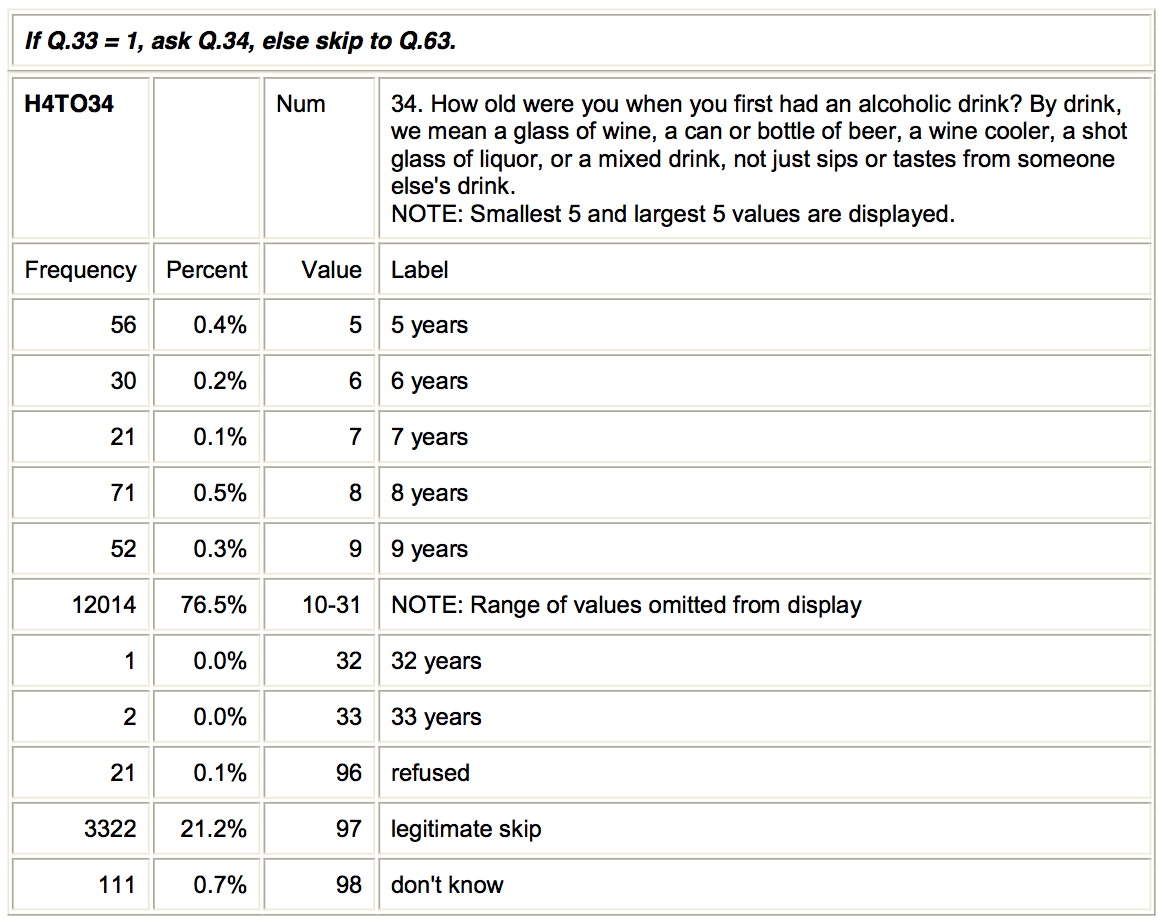
\includegraphics[width=3.5in]{h4to34_codebook.png}
      \end{center}
    \end{frame}

    \begin{frame}[fragile]
\begin{knitrout}
\definecolor{shadecolor}{rgb}{0.137, 0.137, 0.137}\color{fgcolor}\begin{kframe}
\begin{alltt}
\hlstd{drinking}\hlopt{$}\hlstd{age[drinking}\hlopt{$}\hlstd{age} \hlopt{>=} \hlnum{96}\hlstd{]} \hlkwb{<-} \hlnum{NA}
\hlkwd{hist}\hlstd{(drinking}\hlopt{$}\hlstd{age,} \hlkwc{main}\hlstd{=}\hlstr{''}\hlstd{,} \hlkwc{xlab}\hlstd{=}\hlstr{''}\hlstd{,} \hlkwc{col}\hlstd{=}\hlstr{"orange"}\hlstd{)}
\end{alltt}
\end{kframe}
\includegraphics[width=\maxwidth]{/tmp/figures/unnamed-chunk-5-1} 

\end{knitrout}
    \end{frame}

    \begin{frame}{Let's examine our variables using the codebook}
      \begin{center}
        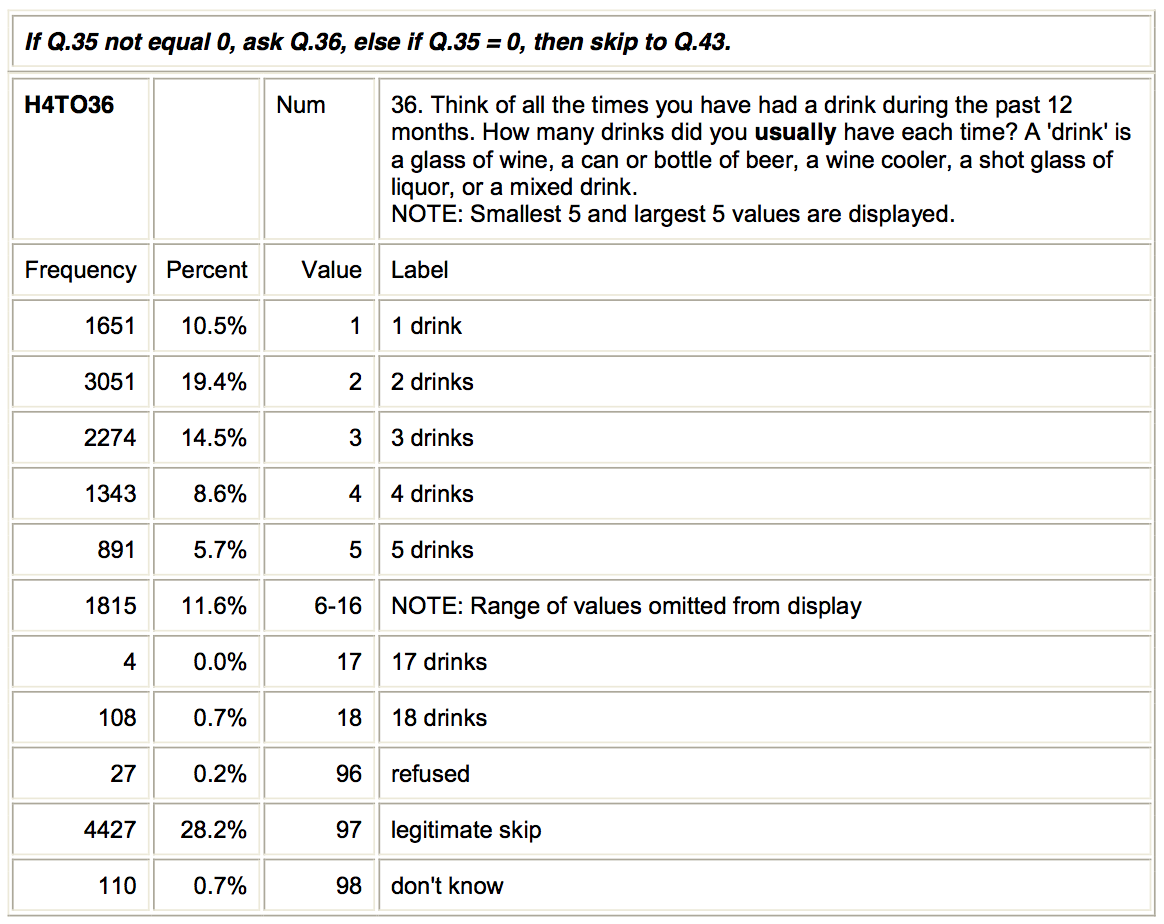
\includegraphics[width=3.5in]{h4to36_codebook.png}
      \end{center}
    \end{frame}

    \begin{frame}[fragile]
\begin{knitrout}
\definecolor{shadecolor}{rgb}{0.137, 0.137, 0.137}\color{fgcolor}\begin{kframe}
\begin{alltt}
\hlstd{drinking}\hlopt{$}\hlstd{num.drinks[drinking}\hlopt{$}\hlstd{num.drinks} \hlopt{>=} \hlnum{96}\hlstd{]} \hlkwb{<-} \hlnum{NA}
\hlkwd{hist}\hlstd{(drinking}\hlopt{$}\hlstd{num.drinks,} \hlkwc{main}\hlstd{=}\hlstr{''}\hlstd{,} \hlkwc{xlab}\hlstd{=}\hlstr{'How many drinks'}\hlstd{,}
  \hlkwc{col}\hlstd{=}\hlstr{"orange"}\hlstd{)}
\end{alltt}
\end{kframe}
\includegraphics[width=\maxwidth]{/tmp/figures/unnamed-chunk-6-1} 

\end{knitrout}
    \end{frame}


    \begin{frame}[fragile]
\begin{knitrout}
\definecolor{shadecolor}{rgb}{0.137, 0.137, 0.137}\color{fgcolor}\begin{kframe}
\begin{alltt}
\hlkwd{plot}\hlstd{(num.drinks} \hlopt{~} \hlstd{age,} \hlkwc{data}\hlstd{=drinking,} \hlkwc{pch}\hlstd{=}\hlnum{16}\hlstd{,} \hlkwc{col}\hlstd{=}\hlstr{"orange"}\hlstd{,}
  \hlkwc{xlab}\hlstd{=}\hlstr{"Age of first drink"}\hlstd{,}
  \hlkwc{ylab}\hlstd{=}\hlstr{"Number of drinks consumed"}\hlstd{)}
\end{alltt}
\end{kframe}
\includegraphics[width=\maxwidth]{/tmp/figures/unnamed-chunk-7-1} 

\end{knitrout}
    \end{frame}

    \begin{frame}[fragile]
\begin{knitrout}
\definecolor{shadecolor}{rgb}{0.137, 0.137, 0.137}\color{fgcolor}\begin{kframe}
\begin{alltt}
\hlkwd{plot}\hlstd{(}\hlkwd{jitter}\hlstd{(num.drinks,} \hlnum{4}\hlstd{)} \hlopt{~} \hlkwd{jitter}\hlstd{(age,} \hlnum{4}\hlstd{),}
  \hlkwc{data}\hlstd{=drinking,} \hlkwc{pch}\hlstd{=}\hlstr{"."}\hlstd{,} \hlkwc{col}\hlstd{=}\hlstr{"orange"}\hlstd{,}
  \hlkwc{xlab}\hlstd{=}\hlstr{"Age of first drink"}\hlstd{,}
  \hlkwc{ylab}\hlstd{=}\hlstr{"Number of drinks consumed"}\hlstd{)}
\end{alltt}
\end{kframe}
\includegraphics[width=\maxwidth]{/tmp/figures/unnamed-chunk-8-1} 

\end{knitrout}
    \end{frame}

    \begin{frame}[fragile]
      The regression line is the line of ``best fit'' through this plot:
\begin{knitrout}
\definecolor{shadecolor}{rgb}{0.137, 0.137, 0.137}\color{fgcolor}
\includegraphics[width=\maxwidth]{/tmp/figures/unnamed-chunk-9-1} 

\end{knitrout}
      
    \end{frame}

    \begin{frame}{What is linear regression doing?}
      We model each case ($x_i=$ age for $i$th person, $y_i=$ number of drinks for $i$th person) as a linear relationship plus some error:
      \[
        y_i = \beta_0 + \beta_1 x_i + \epsilon_i
      \]
      $\beta_0$ and $\beta_1$ are the intercept and slope, respectively.
      \bigskip\pause

      We find estimates for $\beta_0$ and $\beta_1$ in our sample that \emph{minimize} the errors:
      \[
        \hat Y = \hat\beta_0 + \hat\beta_1 X
      \]
      This is the regression (best fit) line.
    \end{frame}

    \begin{frame}{Finding the regression equation}
      When there is just one $X$ variable, the formulas are straightforward:
      \begin{enumerate}
        \item The slope is $\hat\beta_1 = r \cdot \dfrac{\text{SD}(Y)}{\text{SD}(X)}$.
        \item Solve for the intercept using the fact that the regression line will always pass through $(\overline X,\overline Y)$: $\hat\beta_0 = \overline Y - \hat\beta_1\overline X$.
      \end{enumerate}
    \end{frame}

    \begin{frame}[fragile]
      \fontsize{9}{9}\selectfont
\begin{knitrout}
\definecolor{shadecolor}{rgb}{0.137, 0.137, 0.137}\color{fgcolor}\begin{kframe}
\begin{alltt}
\hlstd{model} \hlkwb{<-} \hlkwd{lm}\hlstd{(num.drinks} \hlopt{~} \hlstd{age,} \hlkwc{data}\hlstd{=drinking)}
\hlkwd{summary}\hlstd{(model)}
\end{alltt}
\begin{verbatim}

Call:
lm(formula = num.drinks ~ age, data = drinking)

Residuals:
    Min      1Q  Median      3Q     Max 
-4.2035 -1.8528 -0.8528  0.8095 15.1602 

Coefficients:
            Estimate Std. Error t value Pr(>|t|)    
(Intercept)  6.55417    0.26532   24.70   <2e-16 ***
age         -0.16883    0.01588  -10.63   <2e-16 ***
---
Signif. codes:  0 '***' 0.001 '**' 0.01 '*' 0.05 '.' 0.1 ' ' 1

Residual standard error: 2.963 on 3600 degrees of freedom
  (2902 observations deleted due to missingness)
Multiple R-squared:  0.03044,	Adjusted R-squared:  0.03017 
F-statistic:   113 on 1 and 3600 DF,  p-value: < 2.2e-16
\end{verbatim}
\end{kframe}
\end{knitrout}
      
    \end{frame}

    \begin{frame}[fragile]
      This translates to a regression line of:

      \[
        \widehat{\text{num drinks}} = 6.55 - 0.17 \cdot\text{age}
      \]
      \pause
      Predict number of drinks for $\text{age}=21$:
      \[
        \widehat{\text{num drinks}}
        = 6.55 - 0.17 \cdot 21
        = 3.01
      \]
      Or we can use R to do the work for us:
\begin{knitrout}
\definecolor{shadecolor}{rgb}{0.137, 0.137, 0.137}\color{fgcolor}\begin{kframe}
\begin{alltt}
\hlkwd{predict}\hlstd{(model,} \hlkwd{list}\hlstd{(}\hlkwc{age}\hlstd{=}\hlnum{21}\hlstd{))}
\end{alltt}
\end{kframe}
\end{knitrout}
      
    \end{frame}

    \begin{frame}{How good are our predictions?}
      $R^2$ quantifies how closely the model fits the data.
      \begin{itemize}[<+->]
        \item $R^2$ is the fraction of the variation of $Y$ explained by the model (i.e., $R^2 = \text{Var}(\hat Y)/\text{Var}(Y)$).
        \item $R^2=\text{cor}(X,Y)^2$, i.e., the squared correlation between $X$ and $Y$.
        \item $R^2=0$ when the model has no predictive power at all.
        \item $R^2=1$ when the model yields perfect predictions every time.
        \item $R^2=\text{cor}(Y,\hat Y)^2$, i.e., the squared correlation between the actual and predicted values of $Y$.
      \end{itemize}
    \end{frame}

    \begin{frame}[fragile]
      \fontsize{9}{9}\selectfont
\begin{knitrout}
\definecolor{shadecolor}{rgb}{0.137, 0.137, 0.137}\color{fgcolor}\begin{kframe}
\begin{alltt}
\hlstd{model} \hlkwb{<-} \hlkwd{lm}\hlstd{(num.drinks} \hlopt{~} \hlstd{age,} \hlkwc{data}\hlstd{=drinking)}
\hlkwd{summary}\hlstd{(model)}
\end{alltt}
\begin{verbatim}

Call:
lm(formula = num.drinks ~ age, data = drinking)

Residuals:
   Min     1Q Median     3Q    Max 
-4.204 -1.853 -0.853  0.810 15.160 

Coefficients:
            Estimate Std. Error t value Pr(>|t|)    
(Intercept)   6.5542     0.2653    24.7   <2e-16 ***
age          -0.1688     0.0159   -10.6   <2e-16 ***
---
Signif. codes:  0 '***' 0.001 '**' 0.01 '*' 0.05 '.' 0.1 ' ' 1

Residual standard error: 3 on 3600 degrees of freedom
  (2902 observations deleted due to missingness)
Multiple R-squared:  0.0304,	Adjusted R-squared:  0.0302 
F-statistic:  113 on 1 and 3600 DF,  p-value: <2e-16
\end{verbatim}
\end{kframe}
\end{knitrout}
    \end{frame}

    \begin{frame}
      In our regression, $R^2=0.03$, so $r=\sqrt{0.03}=-0.17$ (negative since the slope is negative).

      \pause\vspace{0.3in}
      Is this ``significant?'' \pause \alert{We'll discuss this next time!}
    \end{frame}

    \section{Regression assumptions}

    \begin{frame}
      In finance, the $\beta$ of an asset indicates its volatility relative to the market. An asset with:
      \pause
      \begin{itemize}[<+->]
        \item $\beta=1$ rises and falls with the market as a whole.
        \item $\beta>1$ is \textbf{more} volatile than the market as a whole.
        \item $\beta<1$ is \textbf{less} volatile than the market as a whole.
      \end{itemize}
      \pause
      $\beta$ is just the slope of the regression line (i.e. $\hat\beta_1$) when we regress the asset's weekly returns against the weekly returns of a market index.
    \end{frame}

    \begin{frame}[fragile]{W5000 (Wilshire 5000, a broad market index)}
\begin{knitrout}
\definecolor{shadecolor}{rgb}{0.137, 0.137, 0.137}\color{fgcolor}\begin{kframe}
\begin{alltt}
\hlkwd{hist}\hlstd{(stock.market}\hlopt{$}\hlstd{W5000,} \hlkwc{col}\hlstd{=}\hlstr{"green"}\hlstd{,} \hlkwc{main}\hlstd{=}\hlstr{""}\hlstd{,}
  \hlkwc{xlab}\hlstd{=}\hlstr{"W5000 return as a % of previous week close"}\hlstd{)}
\end{alltt}
\end{kframe}
\includegraphics[width=\maxwidth]{/tmp/figures/unnamed-chunk-14-1} 

\end{knitrout}
    \end{frame}

    \begin{frame}[fragile]{Amazon (AMZN)}
\begin{knitrout}
\definecolor{shadecolor}{rgb}{0.137, 0.137, 0.137}\color{fgcolor}\begin{kframe}
\begin{alltt}
\hlkwd{plot}\hlstd{(AMZN} \hlopt{~} \hlstd{W5000,} \hlkwc{data}\hlstd{=stock.market,}
  \hlkwc{pch}\hlstd{=}\hlnum{16}\hlstd{,} \hlkwc{col}\hlstd{=}\hlstr{'cyan'}\hlstd{)}
\end{alltt}
\end{kframe}
\includegraphics[width=\maxwidth]{/tmp/figures/unnamed-chunk-15-1} 

\end{knitrout}
    \end{frame}

    \begin{frame}[fragile]
\begin{knitrout}
\definecolor{shadecolor}{rgb}{0.137, 0.137, 0.137}\color{fgcolor}
\includegraphics[width=\maxwidth]{/tmp/figures/unnamed-chunk-16-1} 

\end{knitrout}

      The regression line is
      \[
        \widehat{\text{AMZN}} = 0.4 + 1.13 \cdot\text{W5000},
      \]
      with $R^2=0.22$.
    \end{frame}

    \begin{frame}{Interpreting the regression statistics}
      \begin{itemize}[<+->]
        \item $\hat\beta_1=1.13$ (``$\beta$'') is the predicted increase in returns for AMZN when W5000 returns increase by 1 percentage point---since this is $>1$ AMZN will swing more than the market as a whole
        \item $R^2=0.22$ indicates how closely AMZN tracks W5000 (the market as a whole)
      \end{itemize}
    \end{frame}

    \begin{frame}{Simple regression assumptions}
      We need four things to be true for a regression model to be a good fit for the data:
      \begin{enumerate}
        \item Both $X$ and $Y$ are quantitative
        \item $X$ and $Y$ are approximately linearly related
        \item There are no extreme outliers
        \item The variance of $Y$ is the same for any value of $X$ (``homoscedasticity'')
      \end{enumerate}
    \end{frame}

    \begin{frame}{Simple regression assumptions}
      We need four things to be true for a regression model to be a good fit for the data:
      \begin{enumerate}
        \item Both $X$ and $Y$ are quantitative \greencheckmark
        \item $X$ and $Y$ are approximately linearly related
        \item There are no extreme outliers
        \item The variance of $Y$ is the same for any value of $X$ (``homoscedasticity'')
      \end{enumerate}
    \end{frame}

    \begin{frame}{Assumption 2: Linearity}
      Step 1: Visually examine to ensure a line is a good fit for the data:
\begin{knitrout}
\definecolor{shadecolor}{rgb}{0.137, 0.137, 0.137}\color{fgcolor}
\includegraphics[width=\maxwidth]{/tmp/figures/unnamed-chunk-17-1} 

\end{knitrout}
    \end{frame}

    \begin{frame}{Assumption 2: Linearity}
      Each point has a \textbf{residual} ($Y-\hat Y$); this is the over/under-prediction of the model (red lines).
\begin{knitrout}
\definecolor{shadecolor}{rgb}{0.137, 0.137, 0.137}\color{fgcolor}
\includegraphics[width=\maxwidth]{/tmp/figures/unnamed-chunk-18-1} 

\end{knitrout}
    \end{frame}

    \begin{frame}[fragile]{Assumption 2: Linearity}
      \fontsize{10}{10}\selectfont
      A \textbf{residual plot} (of residuals vs $X$) helps us ensure that there is not subtle nonlinearity. We want to see \textbf{no trend} in this plot:
\begin{knitrout}
\definecolor{shadecolor}{rgb}{0.137, 0.137, 0.137}\color{fgcolor}\begin{kframe}
\begin{alltt}
\hlstd{model} \hlkwb{<-} \hlkwd{lm}\hlstd{(AMZN} \hlopt{~} \hlstd{W5000,} \hlkwc{data}\hlstd{=stock.market)}
\hlkwd{plot}\hlstd{(stock.market}\hlopt{$}\hlstd{W5000,} \hlkwd{resid}\hlstd{(model),}
  \hlkwc{pch}\hlstd{=}\hlnum{16}\hlstd{,} \hlkwc{col}\hlstd{=}\hlstr{"green"}\hlstd{,} \hlkwc{xlab}\hlstd{=}\hlstr{'W5000'}\hlstd{,} \hlkwc{ylab}\hlstd{=}\hlstr{'Residuals'}\hlstd{)}
\end{alltt}
\end{kframe}
\includegraphics[width=\maxwidth]{/tmp/figures/unnamed-chunk-19-1} 

\end{knitrout}
    \end{frame}

    \begin{frame}{Simple regression assumptions}
      We need four things to be true for a regression model to be a good fit for the data:
      \begin{enumerate}
        \item Both $X$ and $Y$ are quantitative \greencheckmark
        \item $X$ and $Y$ are approximately linearly related \greencheckmark
        \item There are no extreme outliers
        \item The variance of $Y$ is the same for any value of $X$ (``homoscedasticity'')
      \end{enumerate}
    \end{frame}

    \begin{frame}[fragile]{Assumption 3: There are no extreme outliers}
      The outliers that would be problematic are those that are \emph{deviate from the existing relationship} between $X$ and $Y$ and are far from the mean on $X$. These would are called \alert{influential points}:
\begin{knitrout}
\definecolor{shadecolor}{rgb}{0.137, 0.137, 0.137}\color{fgcolor}
\includegraphics[width=\maxwidth]{/tmp/figures/unnamed-chunk-20-1} 

\end{knitrout}
    \end{frame}

    \begin{frame}[fragile]{Assumption 3: There are no extreme outliers}
      The outliers that would be problematic are those that are \emph{deviate from the existing relationship} between $X$ and $Y$ and are far from the mean on $X$. These would are called \alert{influential points}:
\begin{knitrout}
\definecolor{shadecolor}{rgb}{0.137, 0.137, 0.137}\color{fgcolor}
\includegraphics[width=\maxwidth]{/tmp/figures/unnamed-chunk-21-1} 

\end{knitrout}
    \end{frame}

    \begin{frame}{Simple regression assumptions}
      We need four things to be true for a regression model to be a good fit for the data:
      \begin{enumerate}
        \item Both $X$ and $Y$ are quantitative \greencheckmark
        \item $X$ and $Y$ are approximately linearly related \greencheckmark
        \item There are no extreme outliers \greencheckmark
        \item The variance of $Y$ is the same for any value of $X$ (``homoscedasticity'')
      \end{enumerate}
    \end{frame}

    \begin{frame}[fragile]{Assumption 4: Homoscedasticity}
      Look for the residual plot to have roughly equal vertical spread all the way across:
\begin{knitrout}
\definecolor{shadecolor}{rgb}{0.137, 0.137, 0.137}\color{fgcolor}
\includegraphics[width=\maxwidth]{/tmp/figures/unnamed-chunk-22-1} 

\end{knitrout}
    \end{frame}

    \begin{frame}{Simple regression assumptions}
      We need four things to be true for a regression model to be a good fit for the data:
      \begin{enumerate}
        \item Both $X$ and $Y$ are quantitative \greencheckmark
        \item $X$ and $Y$ are approximately linearly related \greencheckmark
        \item There are no extreme outliers \greencheckmark
        \item The variance of $Y$ is the same for any value of $X$ (``homoscedasticity'') \greencheckmark
      \end{enumerate}
    \end{frame}

    \begin{frame}{An example where an assumption fails}
      This is a data set of social worker salaries based on years of experience. Which assumption might be violated here?
\begin{knitrout}
\definecolor{shadecolor}{rgb}{0.137, 0.137, 0.137}\color{fgcolor}
\includegraphics[width=\maxwidth]{/tmp/figures/unnamed-chunk-23-1} 

\end{knitrout}
    \end{frame}

    \begin{frame}{An example where an assumption fails}
\begin{knitrout}
\definecolor{shadecolor}{rgb}{0.137, 0.137, 0.137}\color{fgcolor}
\includegraphics[width=\maxwidth]{/tmp/figures/unnamed-chunk-24-1} 

\end{knitrout}
    \end{frame}

    \section{Regression to the mean}

    \begin{frame}
      \fullpagepicture{si}
    \end{frame}
    \begin{frame}
      \fullpagepicture{agt}
    \end{frame}
    \begin{frame}
      \fullpagepicture{sat}
    \end{frame}

    \begin{frame}{What is regression to the mean?}
      \begin{itemize}[<+->]
        \item Whenever two variables are imperfectly related (e.g. first SAT attempt vs second SAT attempt), \alert{regression to the mean} will occur
        \item Extreme cases on one variable (very high or very low scores) will likely be not \emph{quite} so extreme on the other variable, since the good (or bad) luck in the extreme case is not likely to be present the next time around:
          \begin{itemize}[<+->]
            \item If you got a very high SAT score the first time, you probably will score high again, but you probably won't be as lucky the next time around
            \item If you got a very low SAT score the first time, you probably will score poorly again, but you probably won't be as unlucky the next time around
          \end{itemize}
      \end{itemize}
    \end{frame}

    \begin{frame}{What does it have to do with regression?}
      Suppose the correlation between first and second SAT attempts is $r=0.85$, and scores have been standardized, so $\hat Y=0.85 X$:
\begin{knitrout}
\definecolor{shadecolor}{rgb}{0.137, 0.137, 0.137}\color{fgcolor}
\includegraphics[width=\maxwidth]{/tmp/figures/unnamed-chunk-25-1} 

\end{knitrout}
    \end{frame}

    \begin{frame}{What does it have to do with regression?}
      \begin{columns}[onlytextwidth]
        \begin{column}{0.5\textwidth}
          \begin{itemize}[<+->]
            \item $X=2$ (first attempt 2 SD above mean) $\longrightarrow$ $\hat Y = 1.7$ (second attempt 1.7 SD above mean)
            \item $X=0 \longrightarrow \hat Y = 0$ 
            \item $X=-2 \longrightarrow \hat Y = -1.7$
            \item In other words, the second attempts will tend to ``regress'' towards the mean
            \item This has nothing to do with the SAT in particular---it's a statistical phenomenon!
          \end{itemize}
        \end{column}
        \begin{column}{0.5\textwidth}
\begin{knitrout}
\definecolor{shadecolor}{rgb}{0.137, 0.137, 0.137}\color{fgcolor}
\includegraphics[width=\maxwidth]{/tmp/figures/unnamed-chunk-26-1} 

\end{knitrout}
        \end{column}
      \end{columns}
    \end{frame}

  \end{darkframes}

\end{document}
